\documentclass[10pt, aspectratio=169]{beamer}
\usefonttheme{professionalfonts}

\mode<presentation>
{
  \usetheme{Berkeley}
  \usecolortheme{beaver}
  \usefonttheme{default}
  \setbeamertemplate{navigation symbols}{}
  \setbeamertemplate{caption}[numbered]
} 

\setbeamertemplate{footline}{%
  \leavevmode%
  \hbox{%
    \begin{beamercolorbox}[wd=.85\paperwidth,ht=2.5ex,dp=1ex,left]{author in head/foot}%
      \usebeamerfont{author in head/foot}Maxx Seminario, Electronic Circuits, Spring 2026%
    \end{beamercolorbox}%
    \begin{beamercolorbox}[wd=.15\paperwidth,ht=2.5ex,dp=1ex,right]{date in head/foot}%
      \hspace*{0.5em}\insertframenumber{} / \inserttotalframenumber\hspace*{0.5em}%
    \end{beamercolorbox}%
  }%
  \vskip0pt%
}

\usepackage[english]{babel}
\usepackage[utf8x]{inputenc}
\usepackage{tikz}
\usetikzlibrary{shapes.geometric}
\usepackage{pgfplots}
\usepackage{array}
\usepackage{makecell}
\usepackage{verbatim}
\usepackage{graphicx}
\usepackage{subcaption}
\usepackage{amsfonts}
\usepackage{amsmath}
\usepackage{bm}
\usepackage{epstopdf}
\usepackage{circuitikz}
\usepackage{caption}
\usepackage{multirow}
\captionsetup{compatibility=false}
\usepackage[absolute,overlay]{textpos}
\usetikzlibrary{calc}
\usetikzlibrary{pgfplots.fillbetween, backgrounds}
\usetikzlibrary{positioning}
\usetikzlibrary{pgfplots.groupplots}
\usetikzlibrary{plotmarks}
\usetikzlibrary{calc}
\usepgfplotslibrary{groupplots}
\pgfplotsset{compat=newest} 

\usepackage{hyperref}
\definecolor{BeaverRed}{RGB}{179,38,38} 
\hypersetup{
    colorlinks=true,
    linkcolor=BeaverRed,
    filecolor=magenta,      
    urlcolor=cyan,
}

% Added by Maxx Seminario - for colored icons in itemize labels
\usepackage{wasysym} 
\newcommand{\neutralface}{%
  \tikz[baseline=-0.6ex]{
    \draw (0,0) circle (0.9ex);
    \fill (-0.35ex,0.25ex) circle (0.12ex);
    \fill ( 0.35ex,0.25ex) circle (0.12ex);
    \draw (-0.35ex,-0.25ex) -- (0.35ex,-0.25ex);
  }%
}

\newcommand{\baditem}{\textcolor{red! 70! black}{\frownie}}
\newcommand{\gooditem}{\textcolor{green!60!black}{\smiley}}
\newcommand{\mehitem}{\textcolor{orange!80!black}{\neutralface}}

% =========================
% Solution toggle 
% =========================
\newif\ifshowsolutions
\showsolutionstrue   %  compile WITH solutions
%\showsolutionsfalse %  compile WITHOUT solutions

% =========================
% Document Information
% =========================
\title[Semiconductor Physics]{Introduction to Semiconductor Physics}
\subtitle{Crystal Structure, Energy Bands, and Doping}
\author{Maxx Seminario}
\institute{University of Nebraska-Lincoln}
\date{Spring 2026}

\begin{document}

\begin{frame}
  \titlepage
\end{frame}

\section{Introduction}

\begin{frame}{Why Study Semiconductors?}
    
    \begin{columns}[t]
    \column{0.48\textwidth}
        \textbf{Foundation of Modern Electronics}: 
        
        \vspace{0.3cm}
        
        \begin{itemize}
            \item Diodes, transistors, and integrated circuits
            \item Between conductors and insulators
            \item Controllable electrical properties
        \end{itemize}
        
        \vspace{0.5cm}
        
        \textbf{Key Questions}:
        \begin{itemize}
            \item What makes silicon special? 
            \item How do electrons move in semiconductors?
            \item What are energy bands?
            \item How does doping change conductivity?
        \end{itemize}
        
    \column{0.48\textwidth}
        \textbf{Applications}:
        \begin{itemize}
            \item Microprocessors and memory
            \item Sensors and photodetectors
            \item Power electronics
            \item RF and communication devices
        \end{itemize}
        
        \begin{block}{Lecture Objectives}
            \begin{itemize}
                \item Understand crystal structure
                \item Learn about energy bands
                \item Explore intrinsic vs extrinsic semiconductors
                \item Understand n-type and p-type doping
            \end{itemize}
        \end{block}
        
    \end{columns}
    
\end{frame}

\section{Crystal Structure}

\begin{frame}{Types of Materials by Conductivity}
    
    \begin{table}
    \centering
    \renewcommand{\arraystretch}{1.5}
    \begin{tabular}{|l|c|c|l|}
    \hline
    \textbf{Material} & \textbf{Resistivity ($\Omega\cdot$m)} & \textbf{Band Gap (eV)} & \textbf{Examples} \\
    \hline
    \hline
    Conductors & $10^{-8}$ to $10^{-6}$ & 0 & Copper, Aluminum, Gold \\
    \hline
    Semiconductors & $10^{-5}$ to $10^{3}$ & 0.5 to 3 & Silicon, Germanium, GaAs \\
    \hline
    Insulators & $10^{11}$ to $10^{16}$ & $>$ 5 & Glass, Rubber, Diamond \\
    \hline
    \end{tabular}
    \end{table}
    
    \vspace{0.5cm}
    
    \begin{itemize}
        \item \textbf{Conductors}: Many free electrons, low resistance
        \item \textbf{Insulators}: Almost no free electrons, very high resistance
        \item \textbf{Semiconductors}: Few free electrons at room temperature, but controllable ('magic rocks')
    \end{itemize}
    
\end{frame}

\begin{frame}{Silicon Crystal Structure}
    
    \begin{columns}[t]
    \column{0.48\textwidth}
        \textbf{Silicon Atom}:
        \begin{itemize}
            \item Atomic number: 14
            \item 4 valence electrons
            \item Forms covalent bonds
        \end{itemize}
        
        \vspace{0.3cm}
        
        \textbf{Diamond Lattice}:
        \begin{itemize}
            \item Face-centered cubic structure
            \item Each Si atom bonds with 4 neighbors
            \item Tetrahedral arrangement
            \item Very stable at room temperature
        \end{itemize}
        
    \column{0.48\textwidth}
        \begin{center}
        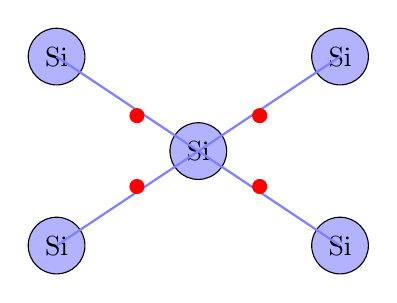
\begin{tikzpicture}[scale=1.2]
            % Central silicon atom
            \draw[fill=blue!30] (0,0) circle (0.3cm) node[black] {Si};
            
            % Four surrounding atoms
            \draw[fill=blue!30] (1.5,1) circle (0.3cm) node[black] {Si};
            \draw[fill=blue!30] (-1.5,1) circle (0.3cm) node[black] {Si};
            \draw[fill=blue!30] (1.5,-1) circle (0.3cm) node[black] {Si};
            \draw[fill=blue!30] (-1.5,-1) circle (0.3cm) node[black] {Si};
            
            % Covalent bonds
            \draw[thick, blue!50] (0,0) -- (1.5,1);
            \draw[thick, blue!50] (0,0) -- (-1.5,1);
            \draw[thick, blue!50] (0,0) -- (1.5,-1);
            \draw[thick, blue!50] (0,0) -- (-1.5,-1);
            
            % Electron pairs on bonds
            \foreach \angle in {30, 150, -30, -150} {
                \fill[red] (0.75*cos \angle, 0.75*sin \angle) circle (0.08cm);
            }
            
        \end{tikzpicture}
        
        \vspace{0.3cm}
        
        \textbf{Covalent Bonding}: Each bond shares 2 electrons
        \end{center}
        
    \end{columns}
    
\end{frame}

\begin{frame}{2D Representation of Silicon Lattice}
    
    \begin{center}
    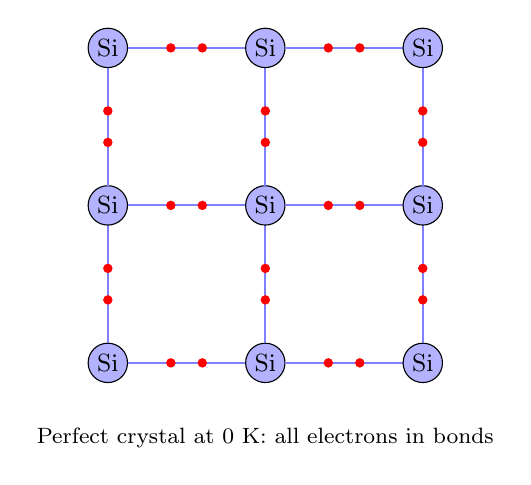
\begin{tikzpicture}[scale=1.0]
        % Draw a 3x3 grid of silicon atoms
        \foreach \x in {0,2,4} {
            \foreach \y in {0,2,4} {
                \draw[fill=blue!30] (\x,\y) circle (0.25cm) node[black, font=\small] {Si};
                
                % Horizontal bonds
                \ifnum\x<4
                    \draw[thick, blue!50] (\x+0.25,\y) -- (\x+1.75,\y);
                    % Electrons on horizontal bonds
                    \fill[red] (\x+0.8,\y) circle (0.06cm);
                    \fill[red] (\x+1.2,\y) circle (0.06cm);
                \fi
                
                % Vertical bonds
                \ifnum\y<4
                    \draw[thick, blue!50] (\x,\y+0.25) -- (\x,\y+1.75);
                    % Electrons on vertical bonds
                    \fill[red] (\x,\y+0.8) circle (0.06cm);
                    \fill[red] (\x,\y+1.2) circle (0.06cm);
                \fi
            }
        }
        
        \node[below, font=\footnotesize] at (2,-0.7) {Perfect crystal at 0 K: all electrons in bonds};
    \end{tikzpicture}
    \end{center}
    
    \vspace{-0.2cm}
    
    \begin{itemize}
        \item At absolute zero (0 K): all valence electrons are bound in covalent bonds
        \item No free electrons $\Rightarrow$ acts as an insulator at 0 K
        \item At room temperature: thermal energy breaks some bonds
    \end{itemize}
    
\end{frame}

\section{Energy Bands}

\begin{frame}{Energy Levels in Atoms vs. Crystals}
    
    \begin{columns}[t]
    \column{0.48\textwidth}
        \textbf{Isolated Silicon Atom}:
        \begin{itemize}
            \item Discrete energy levels
            \item 4 valence electrons
            \item Well-defined orbital energies
        \end{itemize}
        
        \vspace{0.5cm}
        
        \textbf{Silicon Crystal}:
        \begin{itemize}
            \item $\sim 10^{22}$ atoms/cm$^3$
            \item Energy levels merge into bands
            \item Continuous range of energies
        \end{itemize}
        
    \column{0.48\textwidth}
        \begin{center}
        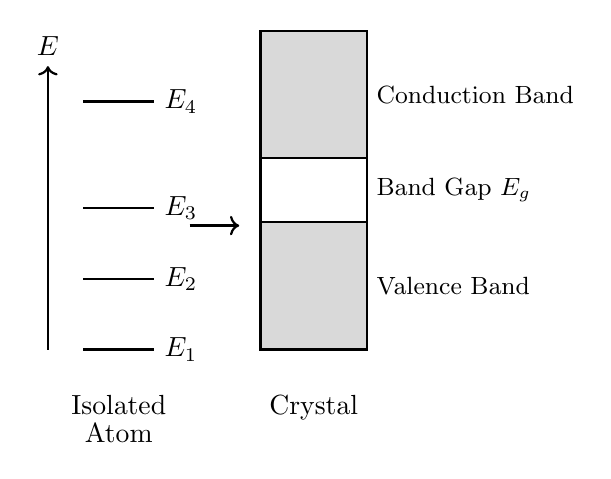
\begin{tikzpicture}[scale=0.9]
            % Energy axis for isolated atoms
            \draw[->, thick] (-0.5,0) -- (-0.5,4) node[above] {$E$};
            
            % Isolated atoms
            \draw[thick] (0,0) -- (1,0) node[right] {$E_1$};
            \draw[thick] (0,1) -- (1,1) node[right] {$E_2$};
            \draw[thick] (0,2) -- (1,2) node[right] {$E_3$};
            \draw[thick] (0,3.5) -- (1,3.5) node[right] {$E_4$};
            \node[below] at (0.5,-0.5) {Isolated};
            \node[below] at (0.5,-0.9) {Atom};
            
            % Arrow
            \draw[->, thick] (1.5,1.75) -- (2.2,1.75);
            
            % Crystal bands
            \draw[thick, fill=gray!30] (2.5,0) rectangle (4,1.8);
            \node[right, font=\small] at (4,0.9) {Valence Band};
            
            \draw[thick, fill=white] (2.5,1.8) rectangle (4,2.7);
            \node[right, font=\small] at (4,2.25) {Band Gap $E_g$};
            
            \draw[thick, fill=gray!30] (2.5,2.7) rectangle (4,4.5);
            \node[right, font=\small] at (4,3.6) {Conduction Band};
            
            \node[below] at (3.25,-0.5) {Crystal};
            
        \end{tikzpicture}
        \end{center}
        
    \end{columns}
    
\end{frame}

\begin{frame}{Energy Band Diagram}
    
    \begin{center}
    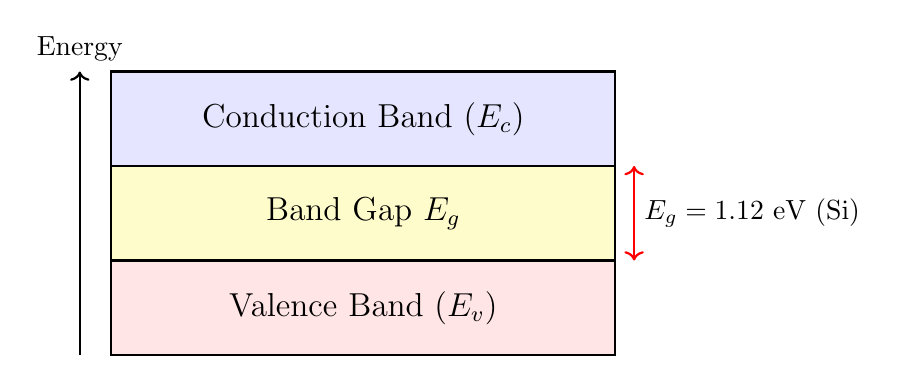
\begin{tikzpicture}[scale=0.8]
        % Conduction Band
        \draw[thick, fill=blue!10] (0,3) rectangle (8,4.5) node[midway, font=\large] {Conduction Band ($E_c$)};
        
        % Band Gap
        \draw[thick, fill=yellow!20] (0,1.5) rectangle (8,3);
        \node[font=\large] at (4,2.25) {Band Gap $E_g$};
        \draw[<->, thick, red] (8.3,1.5) -- (8.3,3) node[midway, right, black] {$E_g = 1.12$ eV (Si)};
        
        % Valence Band
        \draw[thick, fill=red!10] (0,0) rectangle (8,1.5) node[midway, font=\large] {Valence Band ($E_v$)};
        
        % Energy axis
        \draw[->, thick] (-0.5,0) -- (-0.5,4.5) node[above] {Energy};
        
    \end{tikzpicture}
    \end{center}
    
    \vspace{-0.3cm}
    
    \begin{itemize}
        \item \textbf{Valence Band}: Energy levels of bonded electrons
        \item \textbf{Conduction Band}: Energy levels of free electrons
        \item \textbf{Band Gap ($E_g$)}: Energy needed to free an electron from a bond
        \item For silicon: $E_g = 1.12$ eV at room temperature
    \end{itemize}
    
\end{frame}

\begin{frame}{Conductors, Semiconductors, and Insulators}
    
    \begin{center}
    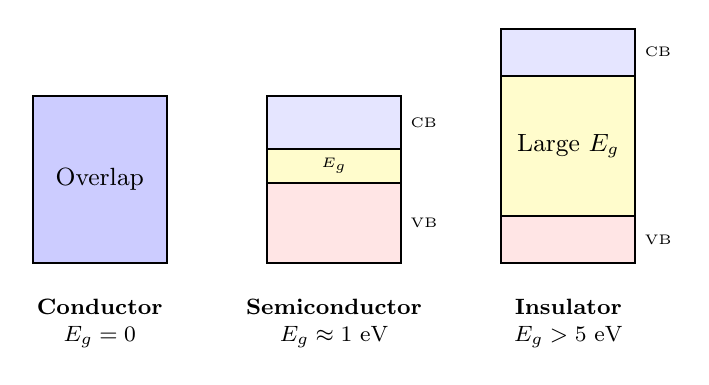
\begin{tikzpicture}[scale=0.85]
        % Conductor
        \begin{scope}[xshift=0cm]
            \draw[thick, fill=blue!20] (0,0) rectangle (2,2.5);
            \node[font=\small] at (1,1.25) {Overlap};
            \node[below, font=\footnotesize] at (1,-0.4) {\textbf{Conductor}};
            \node[below, font=\footnotesize] at (1,-0.8) {$E_g = 0$};
        \end{scope}
        
        % Semiconductor
        \begin{scope}[xshift=3.5cm]
            \draw[thick, fill=blue!10] (0,1.7) rectangle (2,2.5);
            \node[right, font=\tiny] at (2,2.1) {CB};
            \draw[thick, fill=yellow!20] (0,1.2) rectangle (2,1.7);
            \node[font=\tiny] at (1,1.45) {$E_g$};
            \draw[thick, fill=red!10] (0,0) rectangle (2,1.2);
            \node[right, font=\tiny] at (2,0.6) {VB};
            \node[below, font=\footnotesize] at (1,-0.4) {\textbf{Semiconductor}};
            \node[below, font=\footnotesize] at (1,-0.8) {$E_g \approx 1$ eV};
        \end{scope}
        
        % Insulator
        \begin{scope}[xshift=7cm]
            \draw[thick, fill=blue!10] (0,2.8) rectangle (2,3.5);
            \node[right, font=\tiny] at (2,3.15) {CB};
            \draw[thick, fill=yellow!20] (0,0.7) rectangle (2,2.8);
            \node[font=\small] at (1,1.75) {Large $E_g$};
            \draw[thick, fill=red!10] (0,0) rectangle (2,0.7);
            \node[right, font=\tiny] at (2,0.35) {VB};
            \node[below, font=\footnotesize] at (1,-0.4) {\textbf{Insulator}};
            \node[below, font=\footnotesize] at (1,-0.8) {$E_g > 5$ eV};
        \end{scope}
        
    \end{tikzpicture}
    \end{center}
    
    \vspace{0.3cm}
    
    \begin{itemize}
        \item \textbf{Conductors}: Bands overlap, electrons flow easily
        \item \textbf{Semiconductors}: Small band gap, thermally activated conduction
        \item \textbf{Insulators}: Large band gap, very few free electrons
    \end{itemize}
    
\end{frame}

\section{Intrinsic Semiconductors}

\begin{frame}{Electron-Hole Pair Generation}
    
    \begin{columns}[t]
    \column{0.5\textwidth}
        \textbf{Thermal Excitation}:
        \begin{itemize}
            \item At $T > 0$ K, thermal energy breaks bonds
            \item Electron 'jumps' from valence band to conduction band
            \item Leaves behind a \textbf{hole} in valence band
            \item Creates electron-hole pair
        \end{itemize}
        
        \vspace{0.3cm}
        
        \begin{block}{Intrinsic Carrier Concentration}
        $$n_i = p_i \approx 1.5 \times 10^{10} \text{ cm}^{-3}$$
        at 300 K for silicon
        \end{block}
        
    \column{0.48\textwidth}
        \begin{center}
        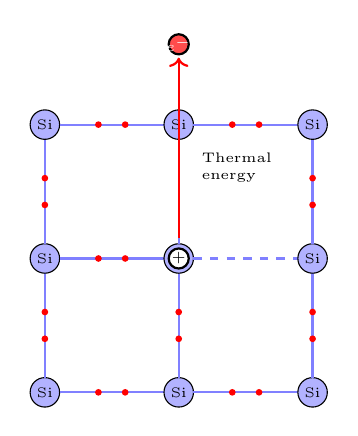
\begin{tikzpicture}[scale=0.85]
            % Lattice with broken bond
            \foreach \x in {0,2,4} {
                \foreach \y in {0,2,4} {
                    \draw[fill=blue!30] (\x,\y) circle (0.22cm) node[black, font=\tiny] {Si};
                    
                    % Horizontal bonds
                    \ifnum\x<4
                        \ifnum\x=2
                            \ifnum\y=2
                                % Broken bond - dashed
                                \draw[thick, blue!50, dashed] (\x+0.22,\y) -- (\x+1.78,\y);
                            \else
                                \draw[thick, blue!50] (\x+0.22,\y) -- (\x+1.78,\y);
                                \fill[red] (\x+0.8,\y) circle (0.05cm);
                                \fill[red] (\x+1.2,\y) circle (0.05cm);
                            \fi
                        \else
                            \draw[thick, blue!50] (\x+0.22,\y) -- (\x+1.78,\y);
                            \fill[red] (\x+0.8,\y) circle (0.05cm);
                            \fill[red] (\x+1.2,\y) circle (0.05cm);
                        \fi
                    \fi
                    
                    % Vertical bonds
                    \ifnum\y<4
                        \ifnum\x=2
                            \ifnum\y=2
                                % Broken bond - dashed
                                \draw[thick, blue!50, dashed] (\x,\y+0.22) -- (\x,\y+1.78);
                            \else
                                \draw[thick, blue!50] (\x,\y+0.22) -- (\x,\y+1.78);
                                \fill[red] (\x,\y+0.8) circle (0.05cm);
                                \fill[red] (\x,\y+1.2) circle (0.05cm);
                            \fi
                        \else
                            \draw[thick, blue!50] (\x,\y+0.22) -- (\x,\y+1.78);
                            \fill[red] (\x,\y+0.8) circle (0.05cm);
                            \fill[red] (\x,\y+1.2) circle (0.05cm);
                        \fi
                    \fi
                }
            }
            
            % Free electron
            \draw[fill=red!70, thick] (2,5.2) circle (0.15cm) node[white, font=\tiny] {$e^-$};
            \draw[->, thick, red] (2,2.3) -- (2,5.0);
            \node[right, font=\tiny] at (2.2,3.5) {Thermal};
            \node[right, font=\tiny] at (2.2,3.2) {energy};
            
            % Hole
            \draw[fill=white, draw=black, thick] (2,2) circle (0.15cm) node[black, font=\tiny] {$+$};
            
        \end{tikzpicture}
        \end{center}
        
    \end{columns}
    
\end{frame}

\begin{frame}{Holes: Positive Charge Carriers}
    
    \begin{columns}[t]
    \column{0.48\textwidth}
        \textbf{What is a Hole?}
        \begin{itemize}
            \item Absence of electron in covalent bond
            \item Acts like positive charge carrier
            \item Can move through crystal
            \item Real concept, not just theoretical
        \end{itemize}
        
        \vspace{0.3cm}
        
        \textbf{Hole Motion}:
        \begin{itemize}
            \item Adjacent electron fills the hole
            \item Creates new hole at previous location
            \item Hole appears to move opposite to electrons
        \end{itemize}
        
    \column{0.48\textwidth}
        \begin{block}{Charge and Current}
            \begin{itemize}
                \item \textbf{Electron}: charge $= -q$, moves toward $+$
                \item \textbf{Hole}: charge $= +q$, moves toward $-$
            \end{itemize}
        \end{block}
        
        \vspace{0.3cm}
        
        \begin{center}
        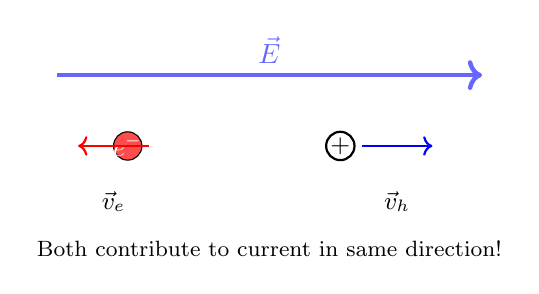
\begin{tikzpicture}[scale=0.9]
            % Electric field
            \draw[->, ultra thick, blue!60] (0,2.5) -- (6,2.5) node[above, midway] {$\vec{E}$};
            
            % Electron motion
            \draw[fill=red!70] (1,1.5) circle (0.2cm) node[white, font=\small] {$e^-$};
            \draw[->, thick, red] (1.3,1.5) -- (0.3,1.5);
            \node[below, font=\small] at (0.8,1.0) {$\vec{v}_e$};
            
            % Hole motion  
            \draw[fill=white, draw=black, thick] (4,1.5) circle (0.2cm) node[black, font=\small] {$+$};
            \draw[->, thick, blue] (4.3,1.5) -- (5.3,1.5);
            \node[below, font=\small] at (4.8,1.0) {$\vec{v}_h$};
            
            % Current direction
            \node[below, font=\footnotesize] at (3,0.3) {Both contribute to current in same direction!};
            
        \end{tikzpicture}
        \end{center}
        
    \end{columns}
    
\end{frame}

\begin{frame}{Intrinsic Semiconductor Properties}
    
    \textbf{Pure (Intrinsic) Semiconductor}:
    \begin{itemize}
        \item No impurities added
        \item Equal number of electrons and holes: $n = p = n_i$
        \item Low conductivity at room temperature
    \end{itemize}
    
    \vspace{-0.3cm}
    
    \begin{center}
    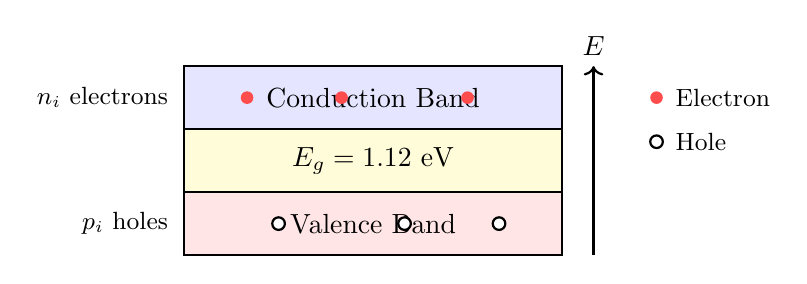
\begin{tikzpicture}[scale=0.8]
        % Energy band diagram
        \draw[thick, fill=blue!10] (0,2.5) rectangle (6,3.5) node[midway] {Conduction Band};
        \draw[thick, fill=yellow!15] (0,1.5) rectangle (6,2.5);
        \node at (3,2) {$E_g = 1.12$ eV};
        \draw[thick, fill=red!10] (0,0.5) rectangle (6,1.5) node[midway] {Valence Band};
        
        % Electrons in CB
        \foreach \x in {1,2.5,4.5} {
            \fill[red!70] (\x,3) circle (0.1cm);
        }
        
        % Holes in VB
        \foreach \x in {1.5,3.5,5} {
            \draw[fill=white, thick] (\x,1) circle (0.1cm);
        }
        
        % Labels
        \node[left, font=\small] at (-0.1,3) {$n_i$ electrons};
        \node[left, font=\small] at (-0.1,1) {$p_i$ holes};
        
        \draw[->, thick] (6.5,0.5) -- (6.5,3.5) node[above] {$E$};
        
        % Legend
        \fill[red!70] (7.5,3) circle (0.1cm);
        \node[right, font=\small] at (7.65,3) {Electron};
        \draw[fill=white, thick] (7.5,2.3) circle (0.1cm);
        \node[right, font=\small] at (7.65,2.3) {Hole};
        
    \end{tikzpicture}
    \end{center}
    
    \vspace{-0.3cm}
    
    \begin{block}{Mass Action Law}
        $$n \cdot p = n_i^2$$
        Valid for both intrinsic and doped semiconductors at thermal equilibrium
    \end{block}
    
\end{frame}

\section{Doped Semiconductors}

\begin{frame}{Why Doping?}
    
    \begin{columns}[t]
    \column{0.48\textwidth}
        \textbf{Problem with Pure Silicon}:
        \begin{itemize}
            \item Very low conductivity
            \item $n_i \approx 10^{10}$ cm$^{-3}$
            \item Compare to Si atoms: $\approx 5 \times 10^{22}$ cm$^{-3}$
            \item Only 1 in $10^{12}$ atoms contributes a charge carrier (electrical current)
        \end{itemize}
        
        \vspace{0.4cm}
        
        \textbf{Solution: Doping}
        \begin{itemize}
            \item Add impurity atoms
            \item Controlled introduction
            \item Typical: 1 dopant per $10^6$ to $10^8$ Si atoms
            \item Increases electrical conductivity
        \end{itemize}
        
    \column{0.48\textwidth}
        \begin{block}{Types of Doping}
            \begin{itemize}
                \item \textbf{n-type}: Add donors (extra electrons)
                \item \textbf{p-type}: Add acceptors (create holes)
            \end{itemize}
        \end{block}
        
        \vspace{0.3cm}
        
        \begin{table}
        \centering
        \renewcommand{\arraystretch}{1.3}
        \small
        \begin{tabular}{|c|c|}
        \hline
        \textbf{Dopant} & \textbf{Type} \\
        \hline
        Phosphorus (P) & n-type \\
        Arsenic (As) & n-type \\
        Antimony (Sb) & n-type \\
        \hline
        Boron (B) & p-type \\
        Aluminum (Al) & p-type \\
        Gallium (Ga) & p-type \\
        \hline
        \end{tabular}
        \end{table}
        
    \end{columns}
    
\end{frame}

\begin{frame}{n-Type Semiconductor (Donor Doping)}
    
    \begin{columns}[t]
    \column{0.5\textwidth}
        \textbf{Adding Phosphorus (P)}:
        \begin{itemize}
            \item P has 5 valence electrons
            \item Si has 4 valence electrons
            \item P substitutes for Si in lattice
            \item 4 electrons form bonds
            \item 5th electron is loosely bound
            \item Easily freed to conduction band
        \end{itemize}
        
        \begin{block}{n-Type Properties}
            \begin{itemize}
                \item $n \gg p$ (electrons dominate)
                \item Electrons = majority carriers
                \item Holes = minority carriers
                \item $n \approx N_D$ (dopant concentration)
            \end{itemize}
        \end{block}
        
    \column{0.48\textwidth}
        \begin{center}
        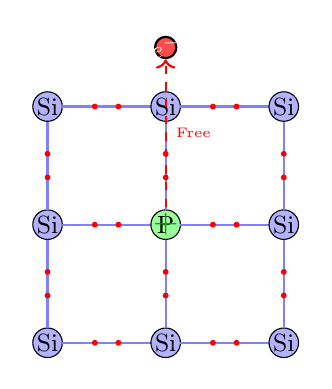
\begin{tikzpicture}[scale=0.75]
            % Lattice with P atom
            \foreach \x in {0,2,4} {
                \foreach \y in {0,2,4} {
                    \ifnum\x=2
                        \ifnum\y=2
                            \draw[fill=green!40] (\x,\y) circle (0.25cm) node[black, font=\small] {P};
                        \else
                            \draw[fill=blue!30] (\x,\y) circle (0.25cm) node[black, font=\small] {Si};
                        \fi
                    \else
                        \draw[fill=blue!30] (\x,\y) circle (0.25cm) node[black, font=\small] {Si};
                    \fi
                    
                    % Bonds
                    \ifnum\x<4
                        \draw[thick, blue!50] (\x+0.25,\y) -- (\x+1.75,\y);
                        \fill[red] (\x+0.8,\y) circle (0.05cm);
                        \fill[red] (\x+1.2,\y) circle (0.05cm);
                    \fi
                    
                    \ifnum\y<4
                        \draw[thick, blue!50] (\x,\y+0.25) -- (\x,\y+1.75);
                        \fill[red] (\x,\y+0.8) circle (0.05cm);
                        \fill[red] (\x,\y+1.2) circle (0.05cm);
                    \fi
                }
            }
            
            % Extra electron from P
            \draw[fill=red!70, thick] (2,5) circle (0.18cm) node[white, font=\small] {$e^-$};
            \draw[->, thick, red, dashed] (2,2.3) -- (2,4.8) node[midway, right, font=\tiny] {Free};
            
            % Positive ion left behind
            \node[font=\large, green!60!black] at (2,2) {$+$};
            
        \end{tikzpicture}
        
        \vspace{0.2cm}
        \small Donor atom donates electron
        \end{center}
        
    \end{columns}
    
\end{frame}

\begin{frame}{p-Type Semiconductor (Acceptor Doping)}
    
    \begin{columns}[t]
    \column{0.5\textwidth}
        \textbf{Adding Boron (B)}:
        \begin{itemize}
            \item B has 3 valence electrons
            \item Si has 4 valence electrons
            \item B substitutes for Si in lattice
            \item Only 3 electrons available for 4 bonds
            \item Creates a hole (missing electron)
            \item Accepts electron from neighboring bond
        \end{itemize}
        
        \begin{block}{p-Type Properties}
            \begin{itemize}
                \item $p \gg n$ (holes dominate)
                \item Holes = majority carriers
                \item Electrons = minority carriers
                \item $p \approx N_A$ (dopant concentration)
            \end{itemize}
        \end{block}
        
    \column{0.48\textwidth}
        \begin{center}
        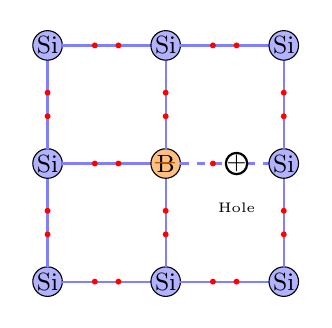
\begin{tikzpicture}[scale=0.75]
            % Lattice with B atom
            \foreach \x in {0,2,4} {
                \foreach \y in {0,2,4} {
                    \ifnum\x=2
                        \ifnum\y=2
                            \draw[fill=orange!50] (\x,\y) circle (0.25cm) node[black, font=\small] {B};
                        \else
                            \draw[fill=blue!30] (\x,\y) circle (0.25cm) node[black, font=\small] {Si};
                        \fi
                    \else
                        \draw[fill=blue!30] (\x,\y) circle (0.25cm) node[black, font=\small] {Si};
                    \fi
                    
                    % Bonds
                    \ifnum\x<4
                        \ifnum\x=2
                            \ifnum\y=2
                                % Missing electron bond
                                \draw[thick, blue!50, dashed] (\x+0.25,\y) -- (\x+1.75,\y);
                                \fill[red] (\x+0.8,\y) circle (0.05cm);
                                % Hole here - no second electron
                            \else
                                \draw[thick, blue!50] (\x+0.25,\y) -- (\x+1.75,\y);
                                \fill[red] (\x+0.8,\y) circle (0.05cm);
                                \fill[red] (\x+1.2,\y) circle (0.05cm);
                            \fi
                        \else
                            \draw[thick, blue!50] (\x+0.25,\y) -- (\x+1.75,\y);
                            \fill[red] (\x+0.8,\y) circle (0.05cm);
                            \fill[red] (\x+1.2,\y) circle (0.05cm);
                        \fi
                    \fi
                    
                    \ifnum\y<4
                        \draw[thick, blue!50] (\x,\y+0.25) -- (\x,\y+1.75);
                        \fill[red] (\x,\y+0.8) circle (0.05cm);
                        \fill[red] (\x,\y+1.2) circle (0.05cm);
                    \fi
                }
            }
            
            % Hole
            \draw[fill=white, draw=black, thick] (3.2,2) circle (0.18cm) node[black, font=\small] {$+$};
            \node[below, font=\tiny] at (3.2,1.5) {Hole};
            
            % Negative ion left behind
            \node[font=\large, orange!70!black] at (2,2) {$-$};
            
        \end{tikzpicture}
        
        \vspace{0.2cm}
        \small Acceptor atom accepts electron (creates hole)
        \end{center}
        
    \end{columns}
    
\end{frame}

\begin{frame}{Energy Band Diagram: Doped Semiconductors}
    
    \begin{columns}[t]
    \column{0.48\textwidth}
        \textbf{n-Type}:
        \begin{center}
        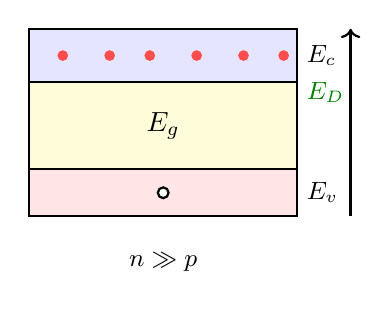
\begin{tikzpicture}[scale=0.85]
            \draw[thick, fill=blue!10] (0,2.5) rectangle (4,3.3);
            \node[right, font=\small] at (4,2.9) {$E_c$};
            
            % Donor level
            \draw[very thick, dashed, green!50!black] (0,2.35) -- (4,2.35);
            \node[right, font=\small, green!50!black] at (4,2.35) {$E_D$};
            
            \draw[thick, fill=yellow!15] (0,1.2) rectangle (4,2.5);
            \node at (2,1.85) {$E_g$};
            
            \draw[thick, fill=red!10] (0,0.5) rectangle (4,1.2);
            \node[right, font=\small] at (4,0.85) {$E_v$};
            
            % Many electrons in CB
            \foreach \x in {0.5,1.2,1.8,2.5,3.2,3.8} {
                \fill[red!70] (\x,2.9) circle (0.08cm);
            }
            
            % Few holes in VB
            \draw[fill=white, thick] (2,0.85) circle (0.08cm);
            
            \draw[->, thick] (4.8,0.5) -- (4.8,3.3);
            
            \node[below, font=\small] at (2,0.1) {$n \gg p$};
        \end{tikzpicture}
        \end{center}
        
        \begin{itemize}
            \item Donor level near $E_c$
            \item Easy to ionize donors
            \item Many electrons in CB
        \end{itemize}
        
    \column{0.48\textwidth}
        \textbf{p-Type}:
        \begin{center}
        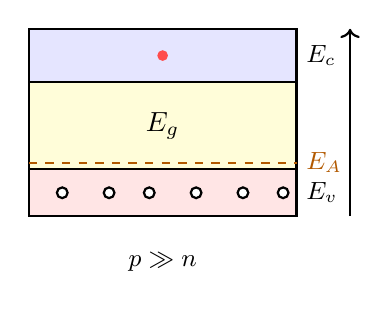
\begin{tikzpicture}[scale=0.85]
            \draw[thick, fill=blue!10] (0,2.5) rectangle (4,3.3);
            \node[right, font=\small] at (4,2.9) {$E_c$};
            
            \draw[thick, fill=yellow!15] (0,1.2) rectangle (4,2.5);
            \node at (2,1.85) {$E_g$};
            
            % Acceptor level
            \draw[thick, dashed, orange!70!black] (0,1.3) -- (4,1.3);
            \node[right, font=\small, orange!70!black] at (4,1.3) {$E_A$};
            
            \draw[thick, fill=red!10] (0,0.5) rectangle (4,1.2);
            \node[right, font=\small] at (4,0.85) {$E_v$};
            
            % Few electrons in CB
            \fill[red!70] (2,2.9) circle (0.08cm);
            
            % Many holes in VB
            \foreach \x in {0.5,1.2,1.8,2.5,3.2,3.8} {
                \draw[fill=white, thick] (\x,0.85) circle (0.08cm);
            }
            
            \draw[->, thick] (4.8,0.5) -- (4.8,3.3);
            
            \node[below, font=\small] at (2,0.1) {$p \gg n$};
        \end{tikzpicture}
        \end{center}
        
        \begin{itemize}
            \item Acceptor level near $E_v$
            \item Easy to ionize acceptors
            \item Many holes in VB
        \end{itemize}
        
    \end{columns}
    
\end{frame}

\section{Current Flow in Semiconductors}

\begin{frame}{Two Mechanisms of Current Flow}
    
    \textbf{1. Drift Current}:
    \begin{itemize}
        \item Caused by electric field
        \item Electrons drift opposite to field, holes drift with field
        \item $J_{drift} = q(n\mu_n + p\mu_p)E$
        \item $\mu_n$, $\mu_p$ are electron and hole mobilities
    \end{itemize}
    
    \textbf{2. Diffusion Current}:
    \begin{itemize}
        \item Caused by concentration gradient
        \item Carriers move from high to low concentration
        \item $J_{diff,n} = qD_n \frac{dn}{dx}$, \quad $J_{diff,p} = -qD_p \frac{dp}{dx}$
        \item $D_n$, $D_p$ are diffusion constants
    \end{itemize}
    
    \begin{block}{Total Current}
        $$J_{total} = J_{drift} + J_{diffusion}$$
        Both mechanisms important in semiconductor devices (especially pn junctions)
    \end{block}
    
\end{frame}

\begin{frame}{Conductivity of Doped Semiconductors}
    
    \textbf{Conductivity Formula}:
    $$\sigma = q(n\mu_n + p\mu_p)$$
    
    \vspace{0.3cm}
    
    \begin{columns}[t]
    \column{0.48\textwidth}
        \textbf{n-Type}:
        \begin{itemize}
            \item $n \approx N_D$ (donor concentration)
            \item $p \ll n$ (minority carriers)
            \item $\sigma \approx qN_D\mu_n$
            \item Conductivity dominated by electrons
        \end{itemize}
        
        \vspace{0.3cm}
        
        \textbf{Example:} $N_D = 10^{16}$ cm$^{-3}$
        \begin{itemize}
            \item 1,000,000 times more carriers than the intrinsic semiconductor
            \item Much higher conductivity
        \end{itemize}
        
    \column{0.48\textwidth}
        \textbf{p-Type}:
        \begin{itemize}
            \item $p \approx N_A$ (acceptor concentration)
            \item $n \ll p$ (minority carriers)
            \item $\sigma \approx qN_A\mu_p$
            \item Conductivity dominated by holes
        \end{itemize}
        
        \vspace{0.3cm}
        
        \textbf{Mass Action Law} still holds:
        $$n \cdot p = n_i^2$$
        
        For n-type: $p = \frac{n_i^2}{N_D}$
        
        For p-type: $n = \frac{n_i^2}{N_A}$
        
    \end{columns}
    
\end{frame}

\begin{frame}{Typical Doping Concentrations}
    
    \begin{table}
    \centering
    \renewcommand{\arraystretch}{1.4}
    \begin{tabular}{|l|c|c|}
    \hline
    \textbf{Type} & \textbf{Concentration (cm$^{-3}$)} & \textbf{Application} \\
    \hline
    \hline
    Intrinsic Si & $n_i = 1.5 \times 10^{10}$ & Reference \\
    \hline
    Lightly doped & $10^{14}$ - $10^{16}$ & Base regions, substrates \\
    \hline
    Moderately doped & $10^{16}$ - $10^{18}$ & Emitter, collector regions \\
    \hline
    Heavily doped & $10^{18}$ - $10^{20}$ & Contacts, low-resistance paths \\
    \hline
    \end{tabular}
    \end{table}
    
    \vspace{0.5cm}
    
    \begin{itemize}
        \item Silicon has $\approx 5 \times 10^{22}$ atoms/cm$^3$
        \item Even "heavy" doping is only $\approx$ 1 dopant per 1000 Si atoms
        \item Precise control needed for device fabrication
        \item Ion implantation and diffusion are common doping techniques
    \end{itemize}
    
\end{frame}

\section{Summary}

\begin{frame}{Key Formulas Reference}
    
    \begin{columns}[T]
    \column{0.48\textwidth}
    \begin{table}[t]
    \centering
    \renewcommand{\arraystretch}{1.8}
    \small
    \begin{tabular}{|l|c|}
    \hline
    \textbf{Parameter} & \textbf{Formula} \\
    \hline
    \hline
    Intrinsic carrier conc. & $n_i \approx 1.5 \times 10^{10}$ cm$^{-3}$ \\
    \hline
    Mass action law & $n \cdot p = n_i^2$ \\
    \hline
    n-type majority & $n \approx N_D$ \\
    \hline
    n-type minority & $p \approx \dfrac{n_i^2}{N_D}$ \\
    \hline
    \end{tabular}
    \end{table}
    
    \column{0.48\textwidth}
    \begin{table}[t]
    \centering
    \renewcommand{\arraystretch}{1.8}
    \small
    \begin{tabular}{|l|c|}
    \hline
    \textbf{Parameter} & \textbf{Formula} \\
    \hline
    \hline
    p-type majority & $p \approx N_A$ \\
    \hline
    p-type minority & $n \approx \dfrac{n_i^2}{N_A}$ \\
    \hline
    Conductivity & $\sigma = q(n\mu_n + p\mu_p)$ \\
    \hline
    Drift current density & $J = \sigma E$ \\
    \hline
    \end{tabular}
    \end{table}
    \end{columns}
    
\end{frame}

\begin{frame}{Summary: Semiconductor Fundamentals}
    
    \begin{enumerate}
        \item \textbf{Crystal Structure}:
        \begin{itemize}
            \item Silicon forms diamond lattice with covalent bonds
            \item 4 valence electrons per atom
        \end{itemize}
        
        \vspace{0.3cm}
        
        \item \textbf{Energy Bands}:
        \begin{itemize}
            \item Valence band (bonded electrons) and conduction band (free electrons)
            \item Band gap $E_g = 1.12$ eV for silicon
            \item Thermal energy creates electron-hole pairs
        \end{itemize}
        
        \vspace{0.3cm}
        
        \item \textbf{Doping}:
        \begin{itemize}
            \item n-type: donor atoms (P, As) provide extra electrons
            \item p-type: acceptor atoms (B, Al) create holes
            \item Dramatically increases conductivity
        \end{itemize}
        
        \vspace{0.3cm}
        
        \item \textbf{Current Mechanisms}:
        \begin{itemize}
            \item Drift (electric field) and diffusion (concentration gradient)
            \item Both important in devices
        \end{itemize}
    \end{enumerate}
    
\end{frame}

\end{document}
